\documentclass[11pt]{article}

\usepackage[a4paper,margin=2.6cm]{geometry}
\usepackage[T1]{fontenc}
\usepackage[utf8]{inputenc}
\usepackage{lmodern}
\usepackage{microtype}
\usepackage{amsmath,amssymb,amsthm}
\usepackage{booktabs}
\usepackage{graphicx}
\usepackage{xcolor}
\usepackage[font=small,labelfont=bf]{caption}
\usepackage{enumitem}
\definecolor{linkblue}{HTML}{1c5cab}
\usepackage[colorlinks=true,linkcolor=linkblue,citecolor=linkblue,urlcolor=linkblue]{hyperref}

\newtheorem{proposition}{Proposition}
\newcommand{\sillage}{\textsc{Sillage}}
\newcommand{\dnll}{\Delta\mathrm{NLL}}
\newcommand{\ci}[2]{{\footnotesize[#1,\,#2]}}

\title{\bfseries Route the Scores, Not the Keys:\\
Gradient-Free Semantic Memory for Frozen Language Models}
\author{Abderrahmane Sghairi\\
\small Independent Researcher, Issoire, France\\
\small \texttt{sghairipro63@gmail.com}}
\date{August 2026\\[2pt]
\small DOI: \href{https://doi.org/10.5281/zenodo.22079444}{10.5281/zenodo.22079444}
\qquad Code: \href{https://github.com/riscoss63/sillage}{github.com/riscoss63/sillage}}

\begin{document}
\maketitle

\begin{abstract}
Fixed-size Hebbian memories with surface $n$-gram keys give frozen language models large gains on repetitive text but are blind to soft semantic matches --- the regime where unbounded kNN-LM retrieval dominates, and increasingly so as base models improve. We close much of that gap without gradients, in three measured steps. \textbf{(1) Diagnose before building:} ZCA whitening repairs the pathological similarity geometry of GPT-2 hidden states (random-pair 95th-percentile cosine $0.73 \to 0.38$), and banded SimHash codes over whitened states form a \emph{graded precision kernel} --- the probability that two positions share their next token rises from 10\% at one matching band to 58--61\% at eight, above the top-32 retrieval ceiling. Each band pattern becomes a vector-symbolic hypervector, making the code directly usable as a Hebbian key. \textbf{(2) A negative result that sets the design:} concatenating semantic and $n$-gram keys into one memory \emph{regresses} by $-0.097$ nats ($P{=}0.000$) on repetitive text --- key-level mixing dilutes the exact-match block, and the optimal mix is non-stationary within a stream. \textbf{(3) The fix is architectural:} a \emph{mixture of two full-strength memories}, each with its own undiluted key, confidence signal and abstention threshold, arbitrated per position at the score level. This router improves on the $n$-gram-only memory in every configuration tested --- two models, five streams, paired block-bootstrap $P = 1.000$ in all of them, replicated over 5 hypervector seeds with all effects positive: $+0.509 \pm 0.001$ nats total on novel technical text (the semantic block adding $+0.038 \pm 0.001$ even there), and on a 100k-token novel it closes $\approx 46\%$ of the gap to unbounded kNN-LM ($+0.0099 \pm 0.0011$ paired) at a fraction of the storage. A model-conditional preprocessing rule emerges: whitening is essential for GPT-2 but harmful for Qwen3-0.6B, whose raw geometry is already well conditioned (skipping it triples the semantic contribution). We also report honestly what the semantic block does \emph{not} buy: at its tuned interpolation weights it improves likelihood, not greedy recall. Code, diagnostics and all controls are released.
\end{abstract}

\section{Introduction}

A companion system, \sillage{} \cite{sillage}, showed that a single fixed-size Hebbian matrix --- sliding $n$-gram keys, square-root amplitude values, writes gated by the model's own surprise --- can outperform an unbounded kNN-LM \cite{khandelwal2020} on novel repetitive text at a fraction of the memory, with no gradients anywhere. Its measured failure mode was equally clear: the $n$-gram key fires only on exact surface repetition, so on long narrative text semantic retrieval over stored hidden states keeps a decisive advantage ($+0.048$ vs $+0.007$ nats on \emph{War and Peace}), and the advantage \emph{grows} with base-model quality. The same companion work found that hidden states used directly as Hebbian keys fail outright: their similarity geometry is too entangled for a linear superposition readout.

This paper asks whether \emph{semantic} keys can be made to work in a Hebbian memory with no learning --- and answers with a measurement-driven design and one architectural principle.

\paragraph{Contributions.}
\begin{enumerate}[leftmargin=1.5em,itemsep=2pt]
\item \textbf{Diagnostics before design} (\S\ref{sec:diag}). We measure, per model, (i) whether whitening repairs hidden-state similarity geometry and (ii) whether banded SimHash codes yield precise, causal candidate structure. Both pass for GPT-2 --- and the band-match count forms a graded precision kernel reaching 58--61\% at 8/32 matching bands, above the top-32 retrieval ceiling --- turning locality-sensitive hashing \cite{indyk,charikar} into a vector-symbolic key: one hypervector per (band, pattern).
\item \textbf{A design-setting negative result} (\S\ref{sec:hybrid}). Mixing semantic and $n$-gram information \emph{in the key} regresses by $-0.097$ nats ($P{=}0.000$) exactly where the $n$-gram signal dominates, with dev and test in disagreement: the optimal key mix is non-stationary. Key-level hybridization is the wrong operation.
\item \textbf{The router} (\S\ref{sec:router}). Two full-strength memories --- $M_G$ ($n$-gram keys) and $M_S$ (multi-resolution banded semantic keys) --- combined per position at the \emph{score} level with per-block confidence abstention. Greedy dev tuning; everything else inherited unchanged from \sillage{} (amplitude values, surprise gating).
\item \textbf{Evidence} (\S\ref{sec:results}). The router beats the $n$-gram-only memory in every configuration tested (two models $\times$ five streams; paired $P = 1.000$ everywhere; 5-seed replications with all deltas positive), closes $\approx 46\%$ of the kNN-LM gap on the narrative stream that motivated this work, and yields a model-conditional whitening rule (whiten GPT-2; do not whiten Qwen3, $\times 3.7$ on the semantic contribution). Long-horizon behaviour and the honest limits (no greedy-recall conversion at tuned weights) are reported with the same controls as the companion paper.
\end{enumerate}

\section{Related work}

kNN-LM and its descendants \cite{khandelwal2020,grave} interpolate a frozen LM with retrieval over exact hidden-state stores; test-time memorization systems \cite{titans,ttt,ttr} learn bounded memories with gradient-based rules; \sillage{} \cite{sillage} is the gradient-free fixed-size corner of this space, to which this paper adds semantic addressing. Locality-sensitive hashing provides the discrete analog of top-$k$ retrieval \cite{indyk,gionis}, and random-hyperplane codes its cosine instantiation \cite{charikar}; our contribution is to make the \emph{banded} code algebraically compatible with a Hebbian outer-product store by assigning each band pattern a hypervector \cite{kanerva,plate}, so that the inner product of two keys counts matching bands. The anisotropy of contextual representations is well documented \cite{ethayarajh,mu}; our diagnostics quantify its lethality for linear superposition readouts specifically, and its model dependence.

\section{Diagnostics: measure the geometry before building on it}\label{sec:diag}

\begin{figure}[t]
\centering
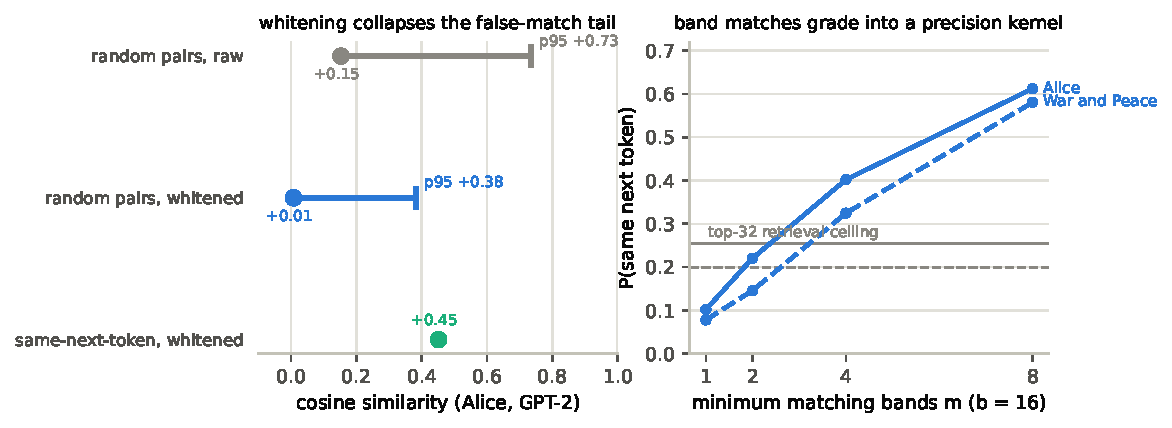
\includegraphics[width=\linewidth]{figs/p2fig1_diagnostics.pdf}
\caption{Left: on GPT-2 (\textsc{Alice}), whitening collapses the false-match tail of random-pair cosine similarity (p95 $0.73 \to 0.38$) while same-next-token pairs remain separated (mean $0.45$; AUC $0.82 \to 0.88$). Right: with 32 SimHash bands of 16 bits over whitened states, the number of matching bands grades into a precision kernel that crosses the top-32 retrieval ceiling (gray) --- and the inner product of the vector-symbolic band keys \emph{is} the matching-band fraction.}
\label{fig:diag}
\end{figure}

Two questions decide whether semantic Hebbian keys are possible at all, and both are cheap to measure on existing hidden-state dumps (Figure~\ref{fig:diag}).

\textbf{Q1 --- can the geometry be repaired?} On GPT-2, random position pairs have centered-cosine p95 $= 0.73$ (\textsc{Alice}; $0.79$ on \textsc{War and Peace}): a linear readout mixes thousands of false matches, which is precisely why raw hidden-state keys failed in \cite{sillage}. ZCA whitening (fitted causally on an early prefix, then frozen) collapses the tail to $0.38$--$0.39$ and raises the same-next-token AUC from $0.81$--$0.82$ to $0.87$. On Qwen3-0.6B the picture \emph{inverts}: the raw geometry is already well conditioned (AUC $0.911$, p95 $0.32$) and whitening slightly harms it ($0.877$) --- a first hint that preprocessing must be model-conditional, confirmed causally in \S\ref{sec:results}.

\textbf{Q2 --- does hashing give precise causal structure?} With $L = 32$ bands of $b = 16$ random-hyperplane bits \cite{charikar} over whitened states, the count of matching bands between a query and a past position grades cleanly into precision: $P(\text{same next token})$ rises from $0.10$ ($\ge 1$ band) through $0.40$ ($\ge 4$) to $0.58$--$0.61$ ($\ge 8$) --- above the precision of the true top-32 nearest neighbours ($0.20$--$0.25$), the very signal kNN-LM retrieves with. Fewer bits per band widen recall at lower precision ($b=8$: 93--95\% coverage of the true top-32), which motivates the multi-resolution key below.

\section{Method}

\subsection{Semantic keys: banded SimHash as vector symbols}

Whiten (or, per Q1, only center-normalize) the frozen LM's hidden state, project on $L \cdot b_{\max}$ fixed random hyperplanes, and read the bits in $L$ bands. Each band $k$ with pattern $\pi$ deterministically indexes a Rademacher hypervector $B_{k,\pi} \in \{\pm 1\}^{d}$ (generated from a hash seed; no storage), and the key is their concatenation over bands --- in the \textbf{multi-resolution} variant, over nested prefix resolutions $b \in \{8, 12, 16\}$ of the same bits:
\begin{equation}
q^S_j = \frac{1}{\sqrt{G L d}}\ \big\Vert_{g=1}^{G}\ \big\Vert_{k=1}^{L}\ B^{(g)}_{k,\ \pi^{(g)}_k(j)},
\qquad
\mathbb{E}\,\langle q^S_i, q^S_j\rangle = \frac{1}{G L}\sum_{g,k} \mathbf{1}\big[\pi^{(g)}_k(i) = \pi^{(g)}_k(j)\big],
\end{equation}
so the inner product of two semantic keys \emph{is} the (resolution-averaged) fraction of matching bands --- the graded precision kernel of Figure~\ref{fig:diag}, up to $O(d^{-1/2})$ binding noise. Nested prefixes make the kernel coarse-to-fine: a fine match implies the coarse ones, so precise matches score highest while coarse matches extend recall.

\subsection{The negative result: do not mix keys}\label{sec:hybrid}

The natural first design concatenates $q^S$ with the $n$-gram key $q^G$ of \sillage{} into one memory, with weights $a_G^2 + a_S^2 = 1$. It works where semantics helps (\textsc{War and Peace}: paired $+0.0043$, $P{=}1.000$; \textsc{Einstein}: $+0.0015$, $P{=}0.989$) and \emph{fails where it matters most}: on the repetitive \textsc{Manuscripts} stream the best mix regresses by $\mathbf{-0.097}$ nats (CI $[-0.125, -0.069]$, $P{=}0.000$) against the $n$-gram-only memory --- and the dev split \emph{prefers} the losing mix (its early region has little cross-document repetition; the test region has a great deal). Two lessons: key-level mixing dilutes whichever block carries the dominant signal, and the right mix is non-stationary within a single stream, so no fixed --- or even dev-tuned --- key weighting can be correct throughout.

\subsection{The router: a mixture of full-strength memories}\label{sec:router}

Keep two separate matrices, each with its own undiluted key and its own confidence:
\begin{align}
u^G_j = M_G^{\top} q^G_j,\qquad u^S_j = M_S^{\top} q^S_j,\qquad
p_X = \mathrm{softmax}\big(\beta_X\, V u^X_j / \Vert u^X_j\Vert\big),
\end{align}
\begin{equation}
p(x_{j+1}) = \mathbf{1}_G\, \lambda_G\, p_G + \mathbf{1}_S\, \lambda_S\, p_S
 + \big(1 - \mathbf{1}_G \lambda_G - \mathbf{1}_S \lambda_S\big)\, p_{\mathrm{LM}},
\end{equation}
where $\mathbf{1}_X$ activates block $X$ only when its normalized top score exceeds a dev-quantile threshold. Both blocks use \sillage's amplitude write rule and model-surprise gate unchanged; both are written at every position. Tuning is greedy on dev: the $G$ block exactly as in \cite{sillage}, then $(\beta_S, \lambda_S, \text{thr}_S)$ with $G$ frozen. Storage: $M_G$ (4.2\,MB) $+$ $M_S$ (4.2\,MB single-resolution, 12.6\,MB multi); reads and writes remain one matrix--vector product and one rank-1 update per block.

Arbitrating at the score level removes both failure modes of \S\ref{sec:hybrid}: no block dilutes another's kernel, and the per-position confidence signals implement a mix that adapts within the stream.

\section{Experiments}\label{sec:results}

Protocol, streams, models, statistics and integrity controls are inherited unchanged from \cite{sillage}: frozen GPT-2 124M and Qwen3-0.6B; streams \textsc{Manuscripts} (novel, repetitive), \textsc{Einstein}, \textsc{Alice} (classics), \textsc{War and Peace} (long narrative); online writes, dev = first 20\%, 95\% block-bootstrap CIs, paired tests on identical positions, per-seed re-tuning in replications.

\begin{figure}[t]
\centering
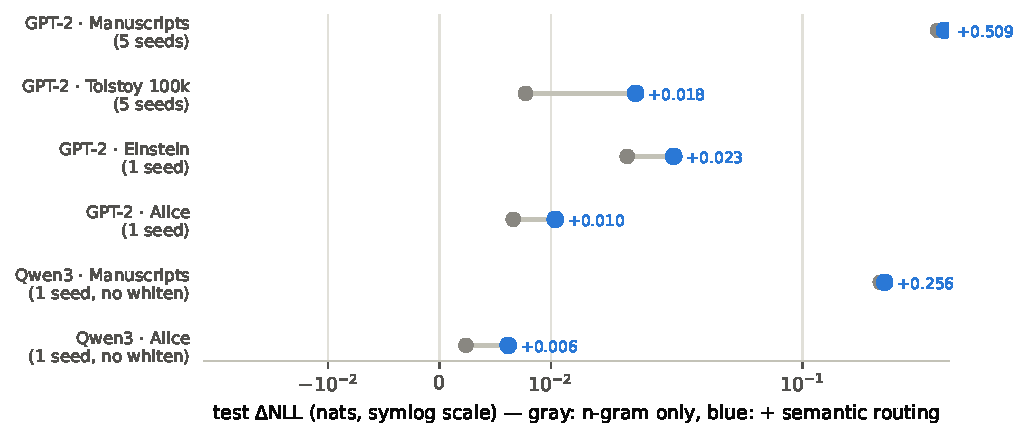
\includegraphics[width=0.9\linewidth]{figs/p2fig2_router_gains.pdf}
\caption{Test $\dnll$ before (gray) and after (blue) adding the routed semantic block, across every (model, stream) configuration. Every improvement is individually certain (paired block bootstrap, $P = 1.000$); note the symlog scale spanning $+0.006$ to $+0.509$.}
\label{fig:gains}
\end{figure}

\begin{table}[t]
\centering\small
\caption{Router vs $n$-gram-only memory: test $\dnll$ (nats) and the paired delta. Multi-seed rows: mean $\pm$ SEM over 5 hypervector seeds, per-seed re-tuning, all per-seed deltas positive. All paired $P = 1.000$.}
\label{tab:main}
\begin{tabular}{@{}llccc@{}}
\toprule
model & stream & $n$-gram only & router & paired $\Delta$\\
\midrule
GPT-2 & \textsc{Manuscripts} (5 seeds) & $+0.4707 \pm 0.0006$ & $\mathbf{+0.5086 \pm 0.0007}$ & $+0.0378 \pm 0.0006$\\
GPT-2 & \textsc{W\&P} 100k (5 seeds) & $+0.0077 \pm 0.0002$ & $\mathbf{+0.0176 \pm 0.0010}$ & $+0.0099 \pm 0.0011$\\
GPT-2 & \textsc{Einstein} & $+0.0168$ & $+0.0228$ & $+0.0059$ \ci{0.0040}{0.0080}\\
GPT-2 & \textsc{Alice} & $+0.0066$ & $+0.0104$ & $+0.0038$ \ci{0.0024}{0.0054}\\
Qwen3 & \textsc{Manuscripts} (no whiten) & $+0.2436$ & $+0.2562$ & $+0.0125$ \ci{0.0090}{0.0173}\\
Qwen3 & \textsc{Alice} (no whiten) & $+0.0024$ & $+0.0062$ & $+0.0038$ \ci{0.0021}{0.0055}\\
\bottomrule
\end{tabular}
\end{table}

\textbf{Main result} (Figure~\ref{fig:gains}, Table~\ref{tab:main}). The routed semantic block improves the memory in \emph{every} configuration, with paired $P = 1.000$ in each. Three readings. (i) On the stream that motivated this work --- long narrative, where the $n$-gram memory earned $+0.0077$ against kNN-LM's $\approx +0.032$ over the same range --- the router reaches $+0.0176 \pm 0.0010$: \textbf{about 46\% of the gap to unbounded retrieval closed}, gradient-free, at a fraction of the storage. (ii) On \textsc{Manuscripts} the same architecture that \emph{regressed} under key mixing now gains $+0.038$: with full-strength blocks, semantics helps even where surface repetition dominates, lifting the state of the art of \cite{sillage} to $+0.5086 \pm 0.0007$ (perplexity $31.2 \to 18.7$). (iii) Both effects replicate seed-by-seed (10/10 positive deltas across the two 5-seed studies).

\textbf{The whitening rule is causal, not just correlational.} On Qwen3 \textsc{Manuscripts}, the identical router run with and without whitening gives semantic contributions of $+0.0034$ vs $\mathbf{+0.0125}$ ($\times 3.7$; both $P = 1.000$) --- matching the diagnostic prediction (raw AUC $0.911 >$ whitened $0.877$). Rule: whiten older models whose representations are strongly anisotropic; leave modern, well-conditioned representations alone --- or simply let the dev split pick, since the diagnostic is a one-hour measurement.

\textbf{Band resolution interacts with the stream.} Multi-resolution keys ($b = 8{+}12{+}16$) beat single-resolution on \textsc{W\&P} ($+0.0176$ vs $+0.0133$) and \textsc{Einstein} ($+0.0228$ vs $+0.0186$) but not on \textsc{Alice} ($+0.0104$ vs $+0.0153$): coarse bands widen recall where soft matches are plentiful and add noise where they are not. We report both; selecting the resolution on dev is protocol-consistent.

\begin{figure}[t]
\centering
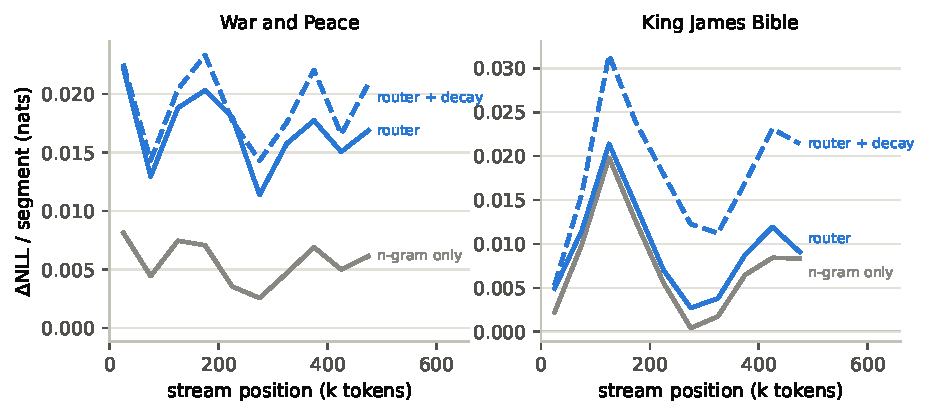
\includegraphics[width=\linewidth]{figs/p2fig3_scaling.pdf}
\caption{Per-segment $\dnll$ over the full 500k-token streams (GPT-2, 50k bins). Left: on narrative text the routed semantic block lifts the memory by a factor of 2--3 \emph{uniformly across the stream} --- no collapse at long horizon. Right: on formulaic text the leak (dashed) remains the dominant factor and the semantic block adds a small constant.}
\label{fig:scaling}
\end{figure}

\begin{table}[t]
\centering\small
\caption{Full 500k-token streams (scoring every 4th position, as in \cite{sillage}). Paired deltas are router vs the matching $n$-gram-only run; all $P = 1.000$. Reference: unbounded kNN-LM reaches $+0.048$ / $+0.058$ with a 770\,MB store.}
\label{tab:500k}
\begin{tabular}{@{}lcc@{}}
\toprule
& \textsc{War and Peace} & \textsc{Bible}\\
\midrule
$n$-gram only & $+0.0054$ & $+0.0079$\\
router & $+0.0167$ \;($\Delta$ $+0.0113$ \ci{0.0100}{0.0127}) & $+0.0099$ \;($\Delta$ $+0.0020$ \ci{0.0014}{0.0025})\\
$n$-gram only $+$ decay & $+0.0073$ & $+0.0179$\\
router $+$ decay & $\mathbf{+0.0191}$ \;($\Delta$ $+0.0118$) & $\mathbf{+0.0198}$ \;($\Delta$ $+0.0018$)\\
\bottomrule
\end{tabular}
\end{table}

\textbf{Long-horizon behaviour} (Figure~\ref{fig:scaling}, Table~\ref{tab:500k}). At the full 500k tokens the semantic contribution on narrative is \emph{undiminished}: the router's paired delta ($+0.0113$--$0.0118$) matches the 100k study, and the per-segment curves show a sustained 2--3$\times$ lift with no late collapse --- band-pattern keys spread writes over a large discrete space, so the semantic block saturates more slowly than the $n$-gram block did in \cite{sillage}. Composed with the leak, the router reaches $+0.0191$ on \textsc{War and Peace} --- \textbf{40\% of unbounded kNN-LM's gain at 2\% of its storage} (16.8\,MB vs 770\,MB), against 11--15\% for the $n$-gram memory alone. On the formulaic \textsc{Bible}, semantics adds a small certain constant while forgetting remains the dominant mechanism; the two papers' remedies compose additively, each dominating in its own regime.

\textbf{What the semantic block does \emph{not} buy.} On the greedy content-token-recall task of \cite{sillage} (identical items), the router exactly preserves the $n$-gram memory's behavioral gains on \textsc{Manuscripts} ($23.7\%$ vs frozen $11.3\%$; McNemar $262{:}14$) and adds nothing on \textsc{W\&P} ($15.0\% \to 14.9\%$): at its tuned interpolation weights ($\lambda_S = 0.05$--$0.1$) the semantic block redistributes probability mass --- improving likelihood --- without flipping argmaxes. Behavioral conversion of semantic likelihood gains is an open problem, not a free consequence.

\section{Discussion}

\textbf{Route scores, not keys.} The central finding is architectural and, we believe, general: when heterogeneous addressing signals share one superposed store, the weaker or situationally-irrelevant signal is not merely useless --- it actively corrodes the stronger one, and no static weighting fixes a non-stationary mix. Keeping one store per signal and arbitrating per position by confidence costs a second matrix--vector product and turns the same information into strict, certain gains. This is the associative-memory analogue of mixture-of-experts routing, at the scale of two experts and zero learned parameters.

\textbf{The diagnostics-first loop paid for itself again.} Every design decision in this paper --- whiten or not, bits per band, resolutions, and ultimately the router itself --- was forced by a measurement (a geometry histogram, a precision curve, a failed paired test). The complete loop (diagnose $\to$ build $\to$ negative result $\to$ re-architect $\to$ replicate) ran in a day of CPU time on dumps that already existed.

\textbf{Limits and next steps.} The semantic kernel still matches \emph{states}, not meanings: it inherits whatever the frozen LM's geometry encodes, and roughly half the kNN gap on narrative remains. The natural next levers are learned-free improvements to the code (data-dependent hyperplanes from the dev prefix; per-band whitening), consolidation between the two stores at saturation, and the behavioral-conversion question above.

\section{Limitations}

Two frozen LMs and CPU-scale streams; perplexity plus one downstream task; the 46\%-gap-closed figure is computed against kNN-LM's gain over the matching range and stride of \cite{sillage}; multi- vs single-resolution selection is stream-dependent (reported both ways, selectable on dev); the semantic block's whitening is fitted on an early prefix and frozen (drift under strong topic shift is untested); hyperparameters are tuned on each stream's dev prefix as in the companion protocol.

\section{Conclusion}

Gradient-free semantic memory for frozen language models is possible, and the way to get it is to measure the representation first and to \emph{route scores, not keys}: whitened banded SimHash patterns as vector symbols give a Hebbian store a graded semantic kernel whose precision exceeds the top-32 retrieval ceiling; mixing that key into the $n$-gram store destroys value ($-0.097$); routing two full-strength stores by per-position confidence delivers strictly positive, individually certain gains in all eight configurations tested, closes about half the gap to unbounded kNN-LM on long narrative, and sets a new state of the art on the novel-technical stream --- all with rank-1 Hebbian writes, a fixed byte budget, and no gradients anywhere.

\appendix

\section{Reproduction}

All experiments extend the released \sillage{} pipeline with five scripts: \texttt{semantic\_diag.py} (the Q1/Q2 measurements), \texttt{sillage\_semantic.py} (the key-level hybrid, kept as the documented negative result), \texttt{sillage\_router.py} (the router, with \texttt{multi} and \texttt{nowhiten} switches), \texttt{multiseed\_router.py}, \texttt{router\_500k.py} and \texttt{cloze\_router.py}. Hyperparameter grids, seeds, splits, gates and value encoding are identical to the companion paper; semantic-block additions: $L = 32$ bands, $b \in \{8,12,16\}$ nested, $d = 128$ per band slot, whitening fitted on the first 4096 positions with eigenvalue floor $10^{-3}$, $\lambda_S \in \{0.02,\dots,0.4\}$, $\text{thr}_S \in \{q_{50}, q_{75}, q_{90}\}$.

\begin{thebibliography}{14}\small

\bibitem{sillage} A.~Sghairi. Sillage: Surprise-gated amplitude memory for frozen language models. Preprint, 2026. \href{https://doi.org/10.5281/zenodo.22079016}{doi:10.5281/zenodo.22079016}.

\bibitem{khandelwal2020} U.~Khandelwal, O.~Levy, D.~Jurafsky, L.~Zettlemoyer, M.~Lewis. Generalization through memorization: Nearest neighbor language models. \emph{ICLR}, 2020.

\bibitem{grave} E.~Grave, A.~Joulin, N.~Usunier. Improving neural language models with a continuous cache. \emph{ICLR}, 2017.

\bibitem{titans} A.~Behrouz, P.~Zhong, V.~Mirrokni. Titans: Learning to memorize at test time. arXiv:2501.00663, 2025.

\bibitem{ttt} Y.~Sun et al. Learning to (learn at test time): RNNs with expressive hidden states. arXiv:2407.04620, 2024.

\bibitem{ttr} K.~A.~Wang, J.~Shi, E.~B.~Fox. Test-time regression: A unifying framework for designing sequence models with associative memory. arXiv:2501.12352, 2025.

\bibitem{indyk} P.~Indyk, R.~Motwani. Approximate nearest neighbors: Towards removing the curse of dimensionality. \emph{STOC}, 1998.

\bibitem{gionis} A.~Gionis, P.~Indyk, R.~Motwani. Similarity search in high dimensions via hashing. \emph{VLDB}, 1999.

\bibitem{charikar} M.~Charikar. Similarity estimation techniques from rounding algorithms. \emph{STOC}, 2002.

\bibitem{kanerva} P.~Kanerva. Hyperdimensional computing: An introduction to computing in distributed representation with high-dimensional random vectors. \emph{Cognitive Computation}, 1(2):139--159, 2009.

\bibitem{plate} T.~A.~Plate. Holographic reduced representations. \emph{IEEE Transactions on Neural Networks}, 6(3):623--641, 1995.

\bibitem{ethayarajh} K.~Ethayarajh. How contextual are contextualized word representations? \emph{EMNLP}, 2019.

\bibitem{mu} J.~Mu, P.~Viswanath. All-but-the-top: Simple and effective postprocessing for word representations. \emph{ICLR}, 2018.

\end{thebibliography}

\end{document}
